\section{Memory}

Applications written for Grappa utilize two forms of memory: local and
global.  Local memory is local to a single core in the system.  Accesses occur
through conventional pointers.  The compiler emits an access and the
memory is manipulated directly.  Applications use local accesses for a
number of things in Grappa: the stack associated with a task, accesses
to localized global memory in caches (see below), and accesses to
debugging infrastructure that is local to each system node.  Local
pointers cannot access memory on other cores, and are valid only on
their home core.

Large data that is expected to be shared and accessed with low locality is
stored in Grappa's global memory. All global data must be accessed through
calls into Grappa's API, shown in Figure~\ref{fig:accessing-memory}.

\paragraph{Global memory addressing} Grappa provides two methods for
storing data in the global memory. The first is a distributed heap
striped across all the machines in the system in a block cyclic fashion.
The \texttt{global\_malloc} and \texttt{global\_free} calls are used to
allocate and deallocate memory in the global heap.  Addresses to memory
in the global heap use \textbf{linear addresses}.  Choosing the block
size involves trading off sequential bandwidth against aggregate random
access bandwidth. Smaller block sizes help spread data across all the
memory controllers in the cluster, but larger block sizes allow the
locality-optimized memory controllers to provide increased sequential
bandwidth. The block size, which is configurable, is typically set to 64
bytes, or the size of a single hardware cache line, in order to exploit
spatial locality when available. The heap metadata is stored on a single
node. Currently all heap operations serialize through this node; while
this has been sufficient for our benchmarks, in the future Grappa will
provide parallel performance through combining~\cite{MAMA,flatcombining}.

Grappa also allows any local data on a core's stacks or heap to be
exported to the global address space to be made accessible to other
cores across the system. Addresses to global memory allocated in this
way use \textbf{2D global addresses}.  This uses a traditional PGAS
addressing model, where each address is a tuple of a rank in the job (or
global process ID) and an address in that process. The lower 48 bits of
the address hold a virtual address in the process. The top bit is set to
indicates that the reference is a 2D address (as opposed to linear
address). This leaves 15 bits for network endpoint ID, which limits our
scalability to $2^{15}$ endpoints. Any node-local data can be made
accessible by other nodes in the system by wrapping the address and node
ID into a 2D global address. This address can then be accessed with a
delegate and can also be cached by other nodes. At the destination the
address is converted into a canonical x86 address by replacing the upper
bits with the sign-extended upper bit of the virtual address. 2D
addresses may refer to memory allocated from a single processes' heap or
from a task's stack. Figure~\ref{fig:memory-structure} shows how 2D and
linear addresses can refer to other cores' memory.


\begin{figure}[htbp]
  \begin{center}
    \begin{description}\small
      \item[ \texttt{ global\_address global\_malloc( size )} ] \hfill \\
      \item[ \texttt{ global\_free( global\_address )} ] \hfill \\
        Allocates and frees memory in the global heap
      \item[ \texttt{ delegate\_read( global\_address, local\_var )} ] 
      \item[ \texttt{ delegate\_write( global\_address, local\_var )} ] %\vspace{-2ex}
      \item[ \texttt{ delegate\_cas( global\_address, local\_var )} ] %\vspace{-2ex}
      \item[ \texttt{ delegate\_fetch\_inc( global\_address, local\_var )} ] %\vspace{-2ex} 
\hfill \\
        Performs a memory operation at the home core of a global address
      \item[ \texttt{ cache\_acquire( global\_address, local\_buf, \{RO,RW,WO\})} ]
      \item[ \texttt{ cache\_release( global\_address, local\_buf )} ] %\vspace{-2ex} 
\hfill \\
Perform cache operations to acquire/release global data.  Acquire, returns a local pointer after all data has been copied to the local node.  Release, optionally writes data back to global memory and frees up management resources.
    \end{description}
    \begin{minipage}{0.95\columnwidth}
      \caption{\label{fig:accessing-memory} Grappa API: accessing memory} %{-4ex}}
    \end{minipage}
    %\vspace{-3ex}
  \end{center}
\end{figure}



\begin{figure}[t]
\begin{center}
  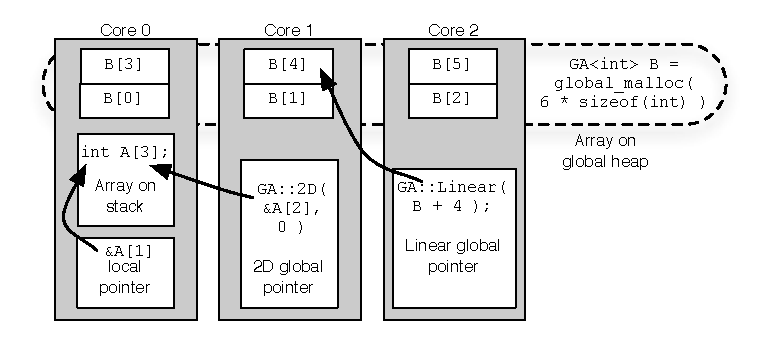
\includegraphics[width=0.95\columnwidth]{figs/memory-structure}
\begin{minipage}{0.95\columnwidth}
  \caption{\label{fig:memory-structure} Grappa memory structure}
\end{minipage}
\vspace{-3ex}
\end{center}
\end{figure}

\paragraph{Global memory access} There are two general approaches
Grappa applications use to {\emph access} global memory. When the
programmer expects a computation on shared data to have spatial locality
to exploit, {\em cache} operations may be used. When there is no
locality to exploit, {\em delegate} operations are used.

\textbf{Explicit caching.} Grappa provides an API to fetch a global
pointer of any length and return a local pointer to a cached copy of the
global memory.  Grappa cache operations have the usual read-only and
read-write variants, along with a write-only variant used to initialize
data structures. Languages for distributed shared memory systems have
done optimizations to achieve a similar goal. For example, the UPC
compiler coalesces struct and array accesses into remote get/put
\cite{Chen:2005}, and Fortran D compiler's message vectorization hoists
small messages out of a loop \cite{FortranD:1992}. Caching in Grappa
additionally provides a mechanism for exploiting temporal locality by
operating on the data locally.
 
Under the hood, Grappa performs the mechanics of gathering chunks of
data from multiple system nodes and presenting a conventional appearing
linear block of memory as a local pointer into a cache. The strategy
employed is to issue all the constituent requests of a cache access
request  (as Active Messages) and then yield until all responses have
occurred.  Currently, Grappa caches are \emph{not} coherent, requiring
the programmer to maintain consistent access to data.  Future work will
develop a software directory based coherence scheme to simplify
consistent access to global data.

\textbf{Delegate operations.} When the access pattern has low-locality,
it is more efficient to modify the data on its home core rather than
bringing a copy to the requesting core and returning it after
modification. Delegate operations provide this capability. Applications
can dispatch computation to be performed on individual machine-word
sized chunks of global memory to the memory system itself (e.g.,
\emph{fetch-and-add}).  Delegate operations, proposed in
\cite{Nelson:hotpar11} and \cite{delegated:oopsla11}, are also the
primary synchronization method in Grappa.

Delegate operations are always executed at the home core of their
address, and while arbitrary memory operations can be delegated, we
restrict the use of delegate operations in three ways to make them more
useful for synchronization. First, we limit each task to one outstanding
delegate operation to avoid the possibility of reordering in the
network. Second, we limit delegate operations to operate on objects in
the 2D address space or objects that fit in a single block of the linear
address space so they can be satisfied with a single network request.
Finally, no context switches are allowed while the data is being
modified. Given these restrictions, we can ensure that delegate
operations for the same address from multiple requesters are always
serialized through a single core in the system, providing atomic
semantics without using atomic operations. 
Figure~\ref{fig:delegate-cache} depicts an example of how delegate and
cache operations interact.

\begin{figure*}[htb]
\begin{center}
  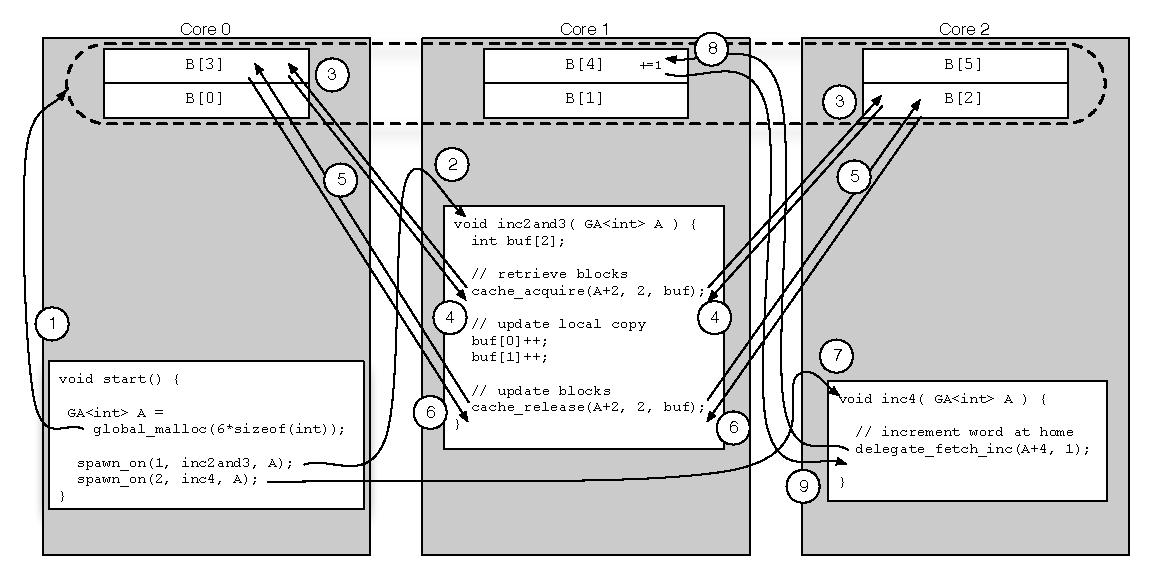
\includegraphics[width=1.5\columnwidth]{figs/delegate-cache}
\begin{minipage}{1.9\columnwidth}
  \caption{\label{fig:delegate-cache} \textbf{Delegation and cache example:} In step 1, a core allocates an array in
the global heap. It then spawns two tasks on remote cores to increment
elements of the array.  The first task increments two elements of the array using cache
operations. In step 2, the task is invoked. A cache request is issued
for two adjacent integers starting at the second element of the
array. Since these element are stored in the memories of two different
cores, this requires the sending of two messages in step 3. The task
is suspended until both responses arrive in step 4. The data carried
in these responses is stored in the local buffer. The elements are
then increment in the buffer. Then in step 5, the modified data is
sent back to the home node. Acknoledgements are returned in step 6 so
the task knows when the writes are complete. The second task increments an element of the array with a delegate
operation. In step 7, the task is invoked. A delegate request is sent
to the home core of the array element with the increment value. The
task suspends until the response is received. In step 8, the increment
is executed on the remote core. A response is returned in step 9 with
the previous value of the array element.
}
\end{minipage}
\vspace{-3ex}
\end{center}
\end{figure*}



